% ===== 原文 pp.25--30（p.30 仅到习题 3.5 结束；§4 标题起见 tr02b） =====

% [原文 p.25]
Coulomb 分支通常还带有一些更为奇异的点，那里的低能动力学不是阿贝尔的。

\subsection{Seiberg--Witten 曲线}

\para{Seiberg--Witten 曲线。} 在 $\fsu(N)=\mathfrak a_{N-1}$ 的情形，我们可以把 $\phi_k$ 的数据用一种几何方式重新打包，即用下面要定义的 SW 曲线 $\Sigma$ 与 SW 微分 $\lambda$。

考虑典范线丛 $T^*C\twoheadrightarrow C$，它在 $C$ 中某一点的纤维由该点处的全体一次形式构成。在 $C$ 的局部坐标 $z$ 下，全空间 $T^*C$ 上有坐标 $(z,x)$，其中 $x\in\C$ 描述一次形式 $x\,\dd z$。存在一个自然嵌入 $C\hookrightarrow T^*C$，即“零截面”，它把 $z\in C$ 映到 $(z,x=0)$。我们把（复）曲线 $\Sigma\subset T^*C$ 定义为满足下式的点 $(z,x)$ 的轨迹：
\begin{equation}
  \left\langle \det(x-\Phi_z)\right\rangle
  = \underbrace{\det(x-\phi_z)}_{\text{见式 (3.14)}}
  = x^N-\sum_{j=2}^{N}u_j(z)\,x^{N-j}=0
  \tag{3.15}
\end{equation}
这里我们用了 $\cO_j$ 的构造 (3.10)，并对 $\fg$ 的每个指数 $j$ 记 $\phi_j=\langle\cO_j\rangle=u_j(z)\dd z^j$。注意 (3.15) 与 $x$ 以及诸 $u_j$ 的变换性质相容，因为其中每一项都是（某个全纯 $N$-形式的唯一分量）。在 $C$ 的一般点 $z\in C$ 处，(3.15) 有 $N$ 个解，这在局部给出 $C$ 的一个 $N$ 重覆盖。一般地，在 $C$ 上某些孤立的点处，两片会以 2 阶分支点相交。如此我们便构造出了 $C$ 的一个 $N$ 重分歧覆盖 $\Sigma$。

% [Tutor Note: p.25 式 (3.15) 的核对办法：取 $N=2$ 时应化为 $x^2-u_2(z)=0$，即 $\phi_2=\frac12\Tr(\phi^2)\dd z^2$ 的特征方程，可与 p.23 的 (3.10)--(3.14) 逐项对照（$\cO_j$ 是 $\phi$ 的第 $j$ 个基本不变式，$\langle\cO_j\rangle=u_j(z)\dd z^j$）。所谓“每一项都是某个全纯 $N$-形式的唯一分量”，是指把 (3.15) 乘以 $\dd z^N$ 后，$x^N\dd z^N$ 与每个 $u_j(z)x^{N-j}\dd z^N$ 都是 $T^*C$ 上的全纯 $N$-形式（$\cO_j$ 是 $j$ 次微分，$x^{N-j}$ 补足余下的 $N-j$ 次），故整条方程在坐标变换下协变。]

正如我们将在具体例子中看到的，$\Sigma$ 恰好是该 4d $\cN=2$ 理论在给定 Coulomb 分支真空上的 SW 曲线，而 SW 微分就是在 $T^*C$ 的坐标 $(z,x)$ 下由 $\lambda=x\,\dd z$ 定义的全纯一次形式。要看出我们的 $(\Sigma,\lambda)$ 与通常的定义相符，在后面的具体理论中会更容易；不过我们可以先给一些直观。除了以间接方式给出低能 $\mathrm{U}(1)^{\dim_\C\cB}$ 矢量多重态所需的预势之外，SW 曲线的任务之一是用粒子的电、磁与味荷来计算其中心荷（从而给出对其质量的 BPS 下界）：这应当通过把 $\lambda$ 沿 $\Sigma$ 中的闭围道积分得到。让我们在 A 型情形下从 M 理论的角度确认这一点。

\para{M 理论视角下的 SW 曲线。} 我们回忆 $\cX(\fsu(N))$ 是 $N$ 张 M5 膜的世界体积理论（已去掉解耦的质心模式）。此时 R 对称性几何地实现为横向的转动。拓扑扭曲对应于把 2d 转动与 2d 横向转动结合起来；于是人们发现，与 $\cX(\fsu(N))$ 在 $\R^{1,3}\times C$ 上作部分扭曲相对应的完整几何设置，是考虑 $\R^{1,3}\times T^*C\times\R^3$ 上的 M 理论，并把 M5 膜沿零截面 $\R^{1,3}\times C$ 放置。\footnote{更一般地，$T^*C$ 可以换成一个四维超 Kähler 流形，而 $C$ 换成 $Q$ 中的全纯闭链。}

走向 Coulomb 分支对应于沿 $T^*C$ 的纤维把 M5 膜彼此移开。由于膜是不可区分的，它们一般会
% [原文 p.26]
重新连成 $C$ 的一个 $N$ 重分歧覆盖 $\Sigma\subset T^*C$。超对称要求它是全纯的，于是我们重现了上面关于 Coulomb 分支真空的分类。我们要强调：UV 曲线 $C$ 刻画的是理论，而 IR 曲线（即 SW 曲线）$\Sigma$ 依赖于（并刻画）给定的 Coulomb 分支真空。

膜系统的激发当然包括 Coulomb 分支上的无质量涨落，但也包括非常有意思的大质量激发，它们来自终止于 M5 膜上的 M2 膜。考虑一个二维曲面 $D\subset T^*C$，其边界落在 SW 曲线上，即 $\partial D\subset\Sigma$；并把一张 M2 膜沿 $D\times\R$ 放置，其中 $\R$ 是 4d 闵可夫斯基空间中的时间方向。从 4d 视角看，这描述一个随时间流逝而静止不动的粒子。它的质量 $m$ 就是 $D$ 的面积，
\begin{equation}
  m=\int_D\left|\dd z\,\dd x\right|
  \ \ge\ \left|\int_D \dd z\,\dd x\right|
  =\left|\int_D \dd(x\,\dd z)\right|
  =\left|\int_{\partial D}\lambda\right|.
  \tag{3.16}
\end{equation}

% [Tutor Note: p.26 式 (3.16) 第二步即 $|\int f|\le\int|f|$（取等号即 BPS 态），第三步用到 $\dd(x\,\dd z)=\dd x\wedge\dd z$ 与 $\dd^2=0$，最后一步用 Stokes 定理。核对要点：$\dd z\,\dd x$ 是 $T^*C$ 上的全纯体积形式，故 $|D|$ 是实的面积；右端只依赖 $\partial D=\gamma$ 在 $\Sigma$ 中的同调类，这正是 SW 微分 $\lambda$ 的周期给出中心荷的来源。]

这与 SW 曲线与微分 $(\Sigma,\lambda)$ 所预期的 BPS 下界相符。事实上，把 SW 曲线 $\Sigma$ 实现为 $C$ 上的纤维化，能比仅仅知道 $\Sigma$（和 $\lambda$）稍微更精细地控制 BPS 谱。确实，$\Sigma$ 上有些闭曲线并不是任何二维曲面 $D\subset T^*C$ 的边界，于是 M 理论的设置“知道”不存在具有这些荷的 BPS 态，而仅凭 $(\Sigma,\lambda)$ 的数据则不知道这一点。

这些 M 理论方面的考虑暗示，我们为 class S 理论找到了正确的 SW 曲线与微分概念。但我们还没有解释 4d 理论的任何具体描述，而只说明了它们在 Coulomb 分支上的 IR 行为。接下来我们就转向这一点。

\subsection{管子与 tinkertoy}

迄今为止我们只讨论了 $\mathrm{T}(\fg,C,D)$ 在其 Coulomb 分支上的低能有效描述。现在我们研究如何在不沿 Coulomb 分支移动的情况下描述 class S 理论。寻找这种描述的向导是：它应当重现上述 IR 物理（它也重现一些受保护的观测量），并且我们找到的不同描述之间应当（严格）相互对偶。回忆部分扭曲保证了我们所关心的 4d 物理只依赖于我们紧化所依据的黎曼面 $C$ 的复结构。因此我们可以选取任何与该复结构相容的度规。

\para{粘合。} 考虑同一个（或不同的）带穿刺点黎曼面 $\overline C$ 上的两个穿刺点 $p_1,p_2\in\overline C$，其中 $C=\overline C\setminus\{p_i\}$，并考虑 $p_1$ 与 $p_2$ 周围的圆盘。就复结构而言，这些带穿刺点的圆盘与半无限圆柱相同，这要归功于指数映照（这里用中心在 $p_i$ 的坐标表示）：
\begin{equation}
  \exp:\ (-\infty,\rho_i]\times\big(\R/(2\pi\Z)\big)
  \ \xrightarrow{\ \sim\ }\ 
  \big\{|z|\le \ee^{\rho_i}\big\}\setminus\{0\}.
  \tag{3.17}
\end{equation}
\begin{center}
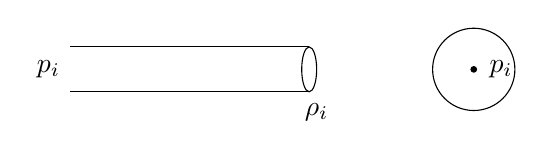
\begin{tikzpicture}[scale=0.95,baseline=(current bounding box.center)]
  \draw (0,0.3)--(3.2,0.3);
  \draw (0,-0.3)--(3.2,-0.3);
  \draw (3.2,0) ellipse (0.1 and 0.3);
  \node[left] at (0,0) {$p_i$};
  \node[below] at (3.3,-0.32) {$\rho_i$};
  \draw (5.4,0) circle (0.55);
  \fill (5.4,0) circle (0.045);
  \node[right] at (5.48,0) {$p_i$};
\end{tikzpicture}
\end{center}

% [Tutor Note: p.26 式 (3.17) 右侧的线描图（柱面沿 $\rho_i$ 截断后与以 $p_i$ 为心的圆盘复结构相同）按 STYLE_GUIDE 6bis 用 TikZ 重画，标签照抄原图。核对：映照把 $w=u+\ii v$（$u\le\rho_i$，$v\sim v+2\pi$）送到 $z=\ee^{w}=\ee^{u}\ee^{\ii v}$，像即是以 $p_i$ 为心、半径 $\ee^{\rho_i}$ 的去心圆盘；$2\pi\Z$ 的周期性与环绕方向相容。]

% [原文 p.27]
我们可以把两个这样的半无限圆柱粘合起来：把它们的无限端在某个有限距离处截掉，并把截断点等同起来，如下图左侧所示：
\begin{equation}
\begin{tikzpicture}[scale=0.85,baseline=(current bounding box.center)]
  \draw (5.9,0) ellipse (2.3 and 1.45);
  \node[align=center] at (6.2,0) {黎曼面的\\其余部分};
  \draw (3.75,0.62)--(0.9,0.62) arc[start angle=90,end angle=270,radius=0.5] -- (3.75,-0.38);
  \draw (3.75,0.3)--(1.3,0.3) arc[start angle=90,end angle=270,radius=0.2] -- (3.75,-0.1);
  \draw (3.75,0.46) ellipse (0.09 and 0.16);
  \draw (3.75,-0.24) ellipse (0.09 and 0.16);
  \draw[dotted] (3.6,0.62)..controls (3.75,0.95) and (3.95,1.02)..(4.2,0.98);
  \draw[dotted] (3.6,-0.38)..controls (3.75,-0.62) and (3.9,-0.66)..(4.1,-0.6);
  \node at (3.95,0.86) {$\rho_1$};
  \node at (3.95,-0.85) {$\rho_2$};
\end{tikzpicture}
\tag{3.18}
\end{equation}
其中“其余部分”在去掉管子后可以仍然连通，也可以变得不连通。用以 $p_1$ 与 $p_2$ 为中心的复坐标 $w$ 与 $z$（$p_1$ 在 $w=0$、$p_2$ 在 $z=0$）表示，这个等同就是
\begin{equation}
  zw=q
  \tag{3.19}
\end{equation}
对某个参数 $q$ 成立。模 $|q|$ 给出管子的长宽比（长度除以周长）$(-\log|q|)/2\pi$，而 $q$ 的相位则表明两个圆柱在粘合前如何相对转动。坐标 $w,z$ 只是局部定义的，因此 $|q|$ 不能太大：管子可以任意长/细，但不能太短/粗，否则这一描述就失效了。

% [Tutor Note: p.27 关于 $|q|$ 的核对：由 (3.19) 的 $zw=q$，把 $w=u+\ii v$、$z=u'+\ii v'$ 代入得 $u+u'=\log|q|$、$v+v'=\arg q$；故“截掉后剩余的柱长”由 $-\log|q|$ 量度，配上周长归一化为 $2\pi$ 后，长度/周长 $=(-\log|q|)/(2\pi)$，与原文一致。原文强调 $|q|$ 不能太大，与“管子不能太短/粗”是同一句话（描述失效）。]

\begin{exercise}{3.3（论带穿刺点的球面）}
1. 在复射影平面 $\C P^1$（二维球面）上取坐标 $w$，其中 $w\in\C\cup\{\infty\}$。对 $n\ge 3$ 个任意互不相同的点 $w_j\in\C\cup\{\infty\}$（$j=1,\dots,n$），定义新坐标 $z(w):=\dfrac{(w-w_1)(w_2-w_3)}{(w-w_3)(w_2-w_1)}$。验证 $w\mapsto z$ 是 $\C P^1$ 上的双射，因而上述定义给出 $\C P^1$ 上的好坐标。验证 $w_1,w_2,w_3$ 分别被映到 $0,1,\infty$。对 $j>3$，$z(w_j)$ 称为 $w_1,w_2,w_3,w_j$ 的交比。

2. 在四孔球面中，当 $w_1,w_2,w_3,w_4$ 作置换时，交比 $q$ 如何变化？

3. 用粘合两个三孔球面 $\C P^1\setminus\{0,1,\infty\}$ 的方式构造四孔球面 $\C P^1\setminus\{0,q,1,\infty\}$。（提示：设 $x,y$ 分别是两个三孔球面上的坐标；在某个区域 $1<|x|<1/|q|$ 上令 $qx=y$。）推广到 $n$ 孔球面。
\end{exercise}
\begin{center}
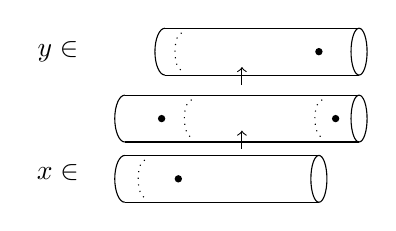
\begin{tikzpicture}[scale=0.85,baseline=(current bounding box.center)]
  \node at (-1.0,1.9) {$y\in$};
  \draw (0.6,2.25)--(3.5,2.25);
  \draw (0.6,1.55)--(3.5,1.55);
  \draw (0.6,2.25) arc[start angle=90,end angle=270,x radius=0.15,y radius=0.35];
  \draw (3.5,1.9) ellipse (0.12 and 0.35);
  \draw[dotted] (0.85,2.18) arc[start angle=90,end angle=270,x radius=0.1,y radius=0.28];
  \fill (2.9,1.9) circle (0.055);
  \draw (0.0,1.25)--(3.5,1.25);
  \draw (0.0,0.55)--(3.5,0.55);
  \draw (0.0,1.25) arc[start angle=90,end angle=270,x radius=0.15,y radius=0.35];
  \draw (3.5,0.9) ellipse (0.12 and 0.35);
  \fill (0.55,0.9) circle (0.055);
  \draw[dotted] (1.0,1.18) arc[start angle=90,end angle=270,x radius=0.11,y radius=0.28];
  \draw[dotted] (2.95,1.18) arc[start angle=90,end angle=270,x radius=0.11,y radius=0.28];
  \fill (3.15,0.9) circle (0.055);
  \node at (-1.0,0.1) {$x\in$};
  \draw (0.0,0.35)--(2.9,0.35);
  \draw (0.0,-0.35)--(2.9,-0.35);
  \draw (0.0,0.35) arc[start angle=90,end angle=270,x radius=0.15,y radius=0.35];
  \draw (2.9,0.0) ellipse (0.12 and 0.35);
  \draw[dotted] (0.3,0.28) arc[start angle=90,end angle=270,x radius=0.1,y radius=0.28];
  \fill (0.8,0.0) circle (0.055);
  \draw[->] (1.75,0.45)--(1.75,0.72);
  \draw[->] (1.75,1.4)--(1.75,1.67);
\end{tikzpicture}
\end{center}

% [Tutor Note: 习题 3.3 后的线描图（两个三孔球面经 $qx=y$ 粘成四孔球面）原文无编号，此处用 TikZ 重画：三条柱面自上而下依次是 $y$ 球面、粘合区、$x$ 球面，细箭头表示两侧的等同。图中虚线弧标出被切掉的圆盘边界，黑点标出穿刺点。]

\para{矢量多重态。} 尽管 (3.18) 画成那样，连接两个穿刺点的圆柱其实是平的，且（对某个度规而言）周长恒为 $2\pi L_5$。我们把沿圆柱方向与绕圆柱方向的坐标分别记为 $x^4,x^5$。我们知道，6d 理论 $\cX(\fg)$ 在圆上约化给出规范代数 $\fg$、耦合 $g_{5d}^2\simeq L_5$ 的 5d $\cN=2$ SYM。因此我们应当预期：把 $\cX(\fg)$ 在粘合曲面 (3.18) 上约化所得到的系统，其中一部分是长度为 $L_4\sim(-\log|q|)L_5$ 的区间上的 5d $\cN=2$ SYM。在 $C$ 收缩为一点
% [原文 p.28]
的极限下，5d 项 $\Tr(F^2)$ 对 $x^4$ 方向的依赖很小，因此 4d 拉格朗日量中应当出现一项
\begin{equation}
  \frac{1}{g_{5d}^2}\int_I \Tr(F^2)=\frac{1}{g_{4d}^2}\Tr(F^2),
  \qquad
  \frac{1}{g_{4d}^2}=\frac{L_4}{g_{5d}^2}\simeq\frac{L_4}{L_5}=-\log|q|.
  \tag{3.20}
\end{equation}

% [Tutor Note: p.28 式 (3.20) 的量纲核对（取质量量纲为 1，故长度量纲为 $-1$）：按标准约定 $[A]=1$、$[F]=2$、$[\Tr F^2]=4$，而 $[g_d^2]=4-d$，即 $[g_{5d}^2]=-1$、$[1/g_{5d}^2]=1$。于是 $(1/g_{5d}^2)\int_I\Tr F^2$ 的量纲为 $1+(-1)+4=4$，恰是 4d 拉格朗日量密度的量纲，与右端 $(1/g_{4d}^2)\Tr(F^2)$（$0+4=4$）一致，故确有 $1/g_{4d}^2=L_4/g_{5d}^2$。再由 $g_{5d}^2\simeq L_5$ 得 $1/g_{4d}^2\simeq L_4/L_5=-\log|q|$；注意 $|q|\to0$ 时 $1/g^2\to+\infty$，即弱耦合，与 (3.22) 的 $\Im\tau=4\pi/g^2>0$ 相符。]

那么 $q$ 的相位呢？它实现沿圆周方向的平移，即绕圆柱的转动。5d 规范场的瞬子流定义为
\begin{equation}
  J^{inst}_\mu=\epsilon_{\mu\nu\rho\sigma\tau}\Tr(F^{\nu\rho}F^{\sigma\tau}).
  \tag{3.21}
\end{equation}
正如我们先前提到的，在从 $\cX(\fg)$ 约化到 5d $\cN=2$ SYM 时，KK（Kaluza--Klein）模式对应于 5d 理论中的瞬子粒子，即 $x^5$ 方向的 KK 动量等于 $J^{inst}$ 下的荷。把 $x^4$ 看作欧氏时间，平移算子 $P_5$ 就由“时间”分量 $J^{inst}_4$ 在 4d“空间”方向 $x^0,\dots,x^3$ 上的积分给出。于是当最终把 $C$ 约化为一点时，把圆柱扭转一个角度 $\theta=\mathrm{Im}\log|q|$ 就为 4d 拉格朗日量贡献一项 $\theta\,\Tr(F\wedge F)$。

% [Tutor Note: p.28 原文此处写 $\theta=\mathrm{Im}\log|q|$，应为 $\theta=\mathrm{Im}\log q$（笔误）：$\log|q|$ 是实数，$\mathrm{Im}\log|q|\equiv0$，而本句与下一句都要求 $\theta$ 是“扭转角”且给出一项 $\theta\Tr(F\wedge F)$；由 (3.22) 的 $\tau=\theta/2\pi+4\pi\ii/g^2$、$q\sim\ee^{2\pi\ii\tau}$ 可反解 $\log q=2\pi\ii\tau$，故 $\theta=2\pi\Re\tau=\mathrm{Im}\log q=\arg q$。译文照印面保留 $\mathrm{Im}\log|q|$，正确形式见本注。]

总的来看，我们预期 (3.18) 中那样的长圆柱应当给出一个 4d $\cN=2$ 矢量多重态，其复化规范耦合 $\tau$ 由 $\log q$ 给出：
\begin{equation}
  \tau=\frac{\theta}{2\pi}+\frac{4\pi\ii}{g^2},
  \qquad
  q\sim \ee^{2\pi\ii\tau}.
  \tag{3.22}
\end{equation}
这一关系在后面的具体几何中会说得更精确。

% [Tutor Note: p.28 式 (3.22) 与 (3.20) 的衔接：$\Im\tau=4\pi/g^2>0$ 自动成立（这正是 p.38「Coupling constants」一段要解释的“为何 $\tau$ 落在上半平面”），而 $\Re\tau=\theta/2\pi$ 对应 $\theta\Tr(F\wedge F)$ 项。核对：$\tau\to\tau+1$ 即 $\theta\to\theta+2\pi$，此时 $q=\ee^{2\pi\ii\tau}$ 不变，与角度 $2\pi$ 周期性相符。]

\para{裤子分解与 S 对偶。} 矢量多重态必须规范化某个物质部分的味对称性，而我们接下来的任务就是理解那份物质来自哪里。为此，关键在于把规范耦合取为零，因为在这个极限下矢量多重态解耦，只剩下带有其味对称性的物质部分。

\begin{exercise}{3.4}
作为一个玩具模型，考虑以群 $G$ 的某个表示变换的标量场 $\phi$，并用规范场 $A$ 把对称性 $G$ 规范化。记 $D=\dd+A$ 为协变导数、$F=\dd A+A\wedge A$，并忽略数值因子。通过引入一个场 $\tilde A=g^{-1}A$（取标准归一化的动能项），证明
\begin{equation}
  \cL=\frac{1}{g^2}\Tr(F^2)+|D\phi|^2
  \ \xrightarrow{\ g\to 0\ }\
  \Tr(\dd\tilde A)^2+|\dd\phi|^2.
  \tag{3.23}
\end{equation}
注意在极限下 $\phi$ 的味对称性 $G$ 不再被规范化。原来的规范理论随后可以通过用一个新的规范场规范化这个味对称性而恢复（只差那个自由的规范场 $\tilde A$）。验证对旋量（$\bar\psi\gamma^\mu D_\mu\psi$）也发生同样的解耦。
\end{exercise}

任何亏格为 $g$、有 $n$ 个穿刺点的带穿刺黎曼面 $C$，除 $(g,n)$ 取 $(0,0),(0,1),(0,2),(1,0)$ 之外，都可以分解为按上述方式粘合的三孔球面（“裤子”）。这样的分解称为裤子分解。对 $C$ 的每个裤子分解，在亏格 $g$、$n$ 个穿刺点的黎曼面的模空间 $\cM_{g,n}$ 中都有一个相应的尖点。在该尖点处，$C$ 被描述为
% [原文 p.29]
由无限细的管子连接的三孔球面。每个这样的管子都给出 4d 理论中一个耦合无限弱的矢量多重态，于是在这个极限下我们可以预期：局域在每个裤子上的 6d 场彼此解耦，因为连接它们的 4d 矢量多重态变成自由的了：
\begin{equation}
\begin{tikzpicture}[scale=0.9,baseline=(current bounding box.center)]
  \draw (0,0) ellipse (1.05 and 0.75);
  \fill (-0.45,0.3) circle (0.055);
  \fill (-0.45,-0.3) circle (0.055);
  \draw (0.95,0.07)--(2.75,0.07);
  \draw (0.95,-0.07)--(2.75,-0.07);
  \draw (0.95,0) ellipse (0.05 and 0.07);
  \draw (2.75,0) ellipse (0.05 and 0.07);
  \node[above] at (1.85,0.12) {自由矢量};
  \draw (3.85,0) ellipse (1.05 and 0.75);
  \fill (3.3,0.3) circle (0.055);
  \fill (3.3,-0.3) circle (0.055);
  \draw (4.8,0.07)--(6.6,0.07);
  \draw (4.8,-0.07)--(6.6,-0.07);
  \draw (4.8,0) ellipse (0.05 and 0.07);
  \draw (6.6,0) ellipse (0.05 and 0.07);
  \node[above] at (5.7,0.12) {自由矢量};
  \draw (7.7,0) ellipse (1.05 and 0.75);
  \fill (7.15,0.3) circle (0.055);
  \fill (7.15,-0.3) circle (0.055);
\end{tikzpicture}
\tag{3.24}
\end{equation}
如同玩具模型那样，被矢量多重态规范化的那些对称性在零耦合极限下恢复为味对称性。

% [Tutor Note: p.29 式 (3.24) 的线描图（每个裤子由一根管子相连，管子收缩时两端多重态变为自由）图内标注两次 “free vector”，此处译为“自由矢量”。核对要点：由 (3.25) 的结构，管子对应规范群 $F\subset F_1\times F_2$，其耦合满足 $1/g^2=-\log|q|\to\infty$（$|q|\to0$），故该矢量多重态自由，与正文“无限弱耦合”一致。]

浮现出来的图景如下。$\mathrm{T}(\fg,C,D)$ 的构件是与三孔球面对应的、称为 tinkertoy 的 class S 理论。这些（4d $\cN=2$）tinkertoy 在每个穿刺点处都有相应的味对称性，我们将在后面仔细研究。对每个管子，考虑它所连接的两个穿刺点各自对应的味对称群 $F_1$ 与 $F_2$，并用一个 4d $\cN=2$ 矢量多重态规范化一个合适的对角子群 $F\subset F_1\times F_2$。这样就得到 $\mathrm{T}(\fg,C,D)$。对 $C$ 的每个裤子分解，$\mathrm{T}(\fg,C,D)$ 的这套描述可以示意地写成
\begin{equation}
  \mathrm{T}(\fg,C,D)
  =\Big(\prod_{\text{裤子}}T(\fg,\text{三孔球面})\Big)
  \Big/\Big(\prod_{\text{管子}}\text{规范群}\Big).
  \tag{3.25}
\end{equation}
理解 AGT 对应的工作中有很大一部分，就是分类由不同类型穿刺点的三孔球面所得到的 tinkertoy。它们的味对称性可以相当复杂，这就是为什么在 (3.25) 中我们不能把规范群写得更具体。

% [Tutor Note: p.29 式 (3.25) 的“商”是说：对每个管子取 $F_1\times F_2$ 的对角子群并规范化，即把相应因子从味对称群中除掉；分子中的 $T(\fg,\text{三孔球面})$ 即每个裤子的 tinkertoy。记号上原文写作 $\mathrm{T}(\fg,\text{sphere}\setminus3\text{pt})$（“球面去掉 3 点”），译文按“三孔球面”处理；$\mathrm{T}$ 是直立体（原文即如此），不要与斜体 $T_\fg$（单一 tinkertoy）混淆。]

当所有穿刺点都是所谓的满驯服穿刺点（后面会解释）时，所有构件都是同一个 tinkertoy $T_\fg$。这个理论是一个孤立的\footnote{一个超对称量给定的 SCFT 称为\textit{孤立的}（isolated），是指它没有任何具有同样超对称的严格边缘形变（例如 4d 中的规范耦合）。} SCFT，带有（至少）与其三个穿刺点相关联的 $\fg^3$ 味对称性。对 $\fg=\fsu(2)$ 它由四个自由超多重态组成，而对其他的 $\fg$ 它没有 4d $\cN=2$ 拉格朗日量描述。

当然，给定的一张黎曼面有许多互不等价的裤子分解。每一种都给出 $\mathrm{T}(\fg,C,D)$ 在参数空间某个角上的弱耦合规范理论描述。在强耦合（短管子）下，另一种描述可能是弱耦合的，因而更为有用。在具体情形中这重现了已知的 4d $\cN=2$ S 对偶。下面是一个用来体会裤子分解的习题。

\begin{exercise}{3.5（裤子分解的组合学）}
1. 给定亏格为 $g$、$n$ 个穿刺点的曲面 $C_{g,n}$，验证所有裤子分解所用到的三孔球面数目相同。

2. 画出四孔球面的三个拓扑上不同\footnote{在此意义下，两个裤子分解相同，是指那些把曲面切成若干带三条边界的碎片的闭曲线可以互相形变，既不自交，也不穿过穿刺点。}的裤子分解（假定穿刺点可区分）。$n$ 孔球面有多少个裤子分解？单孔环面是否有有限个裤子分解？

% [原文 p.30]
3. 回到习题 3.3 的第 3 点，用一切可能的方式粘合三孔球面，构造出 $n=4$（或 5）个穿刺点的球面。

4. 我们不必把黎曼面完全退化到裤子：只要 $C$ 上有一根长管子，理论 $\mathrm{T}(\fg,C,D)$ 就可以写成用一个弱耦合矢量多重态去规范化一个“更小”的 class S 理论的味对称性。那个更小的理论对应什么样的黎曼面（亏格、穿刺点数）？按该曲面去掉管子后是否断开，有两种情形。
\end{exercise}

% 注：习题 3.5 的第 3、4 问在原文 p.30 顶部，故本文件覆盖到 p.30 的这一段为止。
